% Solar Filament Segmentation Challenge 2026 --- team report
% Filled from the official ACM acmart template (guide style off).
% Drop this file (and the figure PNGs) into the organizers' Overleaf project.
% Do not change the black template sentences in the abstract, introduction,
% acknowledgment, or the official references [1] and [2].
\documentclass[sigconf,nonacm]{acmart}

%% Official template switch: gray guide text is off.
\newif\ifguideStyle
\guideStylefalse
\providecommand{\guide}[1]{\ifguideStyle{\color{gray!65}\itshape #1}\fi}

\usepackage{booktabs}
\usepackage{graphicx}
\usepackage{amsmath}
\usepackage{array}

\setcopyright{none}
\settopmatter{printacmref=false, printfolios=false}

\acmConference[Kaggle Competition]{Kaggle Competition}{2026}{kaggle.com/competitions/filament-segmentation-2026}
\acmYear{2026}
\copyrightyear{2026}

\title{U-Net--YOLO Fusion and a Frozen D-FINE-seg Model}
\subtitle{A Solution to the Solar Filament Segmentation Challenge 2026}

\author{James Mills (Brick Bruce)}
\affiliation{%
  \institution{CAGE / Innovative Creative Solutions}
  \city{Port Allen}
  \state{Louisiana}
  \country{United States}
}
\email{arsenalentertainmentinc@gmail.com}

\citestyle{acmnumeric}

% Official-template conference line (local acmart v1.83 + nonacm may omit it).
\fancyfoot[LO,LE]{\fontsize{8}{9}\selectfont\itshape Kaggle Competition, kaggle.com/competitions/filament-segmentation-2026}
\fancyfoot[RO,RE]{\fontsize{8}{9}\selectfont\itshape 2026.}

\emergencystretch=2em
\begin{document}
\begin{abstract}
This report describes our solution to the Solar Filament Segmentation Challenge 2026, a Kaggle competition on automatic segmentation of solar filaments in GONG H-$\alpha$ observations.
We submitted two entries. The first (r13) fuses a semantic U-Net pipeline with a YOLO11s-seg instance model: U-Net instances are kept where YOLO agrees, and small confident YOLO-only filaments are added. On a fresh file-grouped holdout of 201 annotator-images, fusion reached a pooled Panoptic Quality (PQ) of 0.4092 versus 0.3846 for the U-Net alone (gain $+0.0246$; paired per-image bootstrap 95\% lower bound $+0.020$). The second (r16) is a frozen public D-FINE-seg-S model (Apache-2.0). On a leak-free 46-id slice it scored 0.4321 versus 0.4038 for the r13 recipe, but a reuse-adjusted uncertainty gate did not confirm that gain. The file was submitted under an override and scored 0.38 on the public board, against 0.35 for r13.
\end{abstract}

\maketitle


\section{Introduction}
This report goes over the details of our submitted solution to the Solar Filament Segmentation Challenge 2026 [2]. The challenge, launched on July 10, 2026, is organized by the Earth-Space AI Research (ESAIR) Lab\footnote{www.esairlab.com/}. This challenge utilizes the MAGFiLO dataset for evaluation of the segmentation algorithms [1].
The training set has 1,154 annotator-image ids on 707 files ($2048\times2048$ GONG H-$\alpha$ frames) and a 180-image test set. Several annotators can share one file, so every split keeps whole files together. We pre-register each change and score it once on a declared holdout. Code for the r13 pipeline is public.\footnote{\url{https://github.com/brickbruce1975-ship-it/cage-filament-segmentation-2026}}

\section{Methodology}

\paragraph{U-Net + YOLO fusion (r13).}
The semantic branch follows our r5 recipe: two \texttt{segmentation\_models\_pytorch} U-Nets [4] with ResNet34 ImageNet encoders, run on the whole image at 1024\,px with horizontal-flip test-time augmentation (TTA). A \emph{mask} net (22 epochs, seed 5) predicts filament pixels. A \emph{hull} net (16 epochs, seed 6) predicts each filament closed into one blob, with a gap carved between neighbours. Training uses Dice + BCE, AdamW (learning rate $3\times10^{-4}$, weight decay $10^{-4}$), OneCycle (max $10^{-3}$), batch size 4, flip and gain/bias augmentation, and mixed precision. Instances (``config B'') are formed by thresholding the mask at 0.5, grouping mask pixels by hull component (hull threshold 0.3), assigning leftover pixels by a morphological closing of kernel 51, and dropping instances under 250\,px.

The instance branch is Ultralytics YOLO11s-seg [5] at $\mathrm{imgsz}=2048$, 40 epochs, batch 8 on two T4 GPUs, seed 0 (our r10 recipe). Inference uses confidence $\geq 0.05$, NMS 0.7, at most 100 detections, and retina masks.

Fusion follows a recipe frozen after earlier cross-fitting (r12) and not retuned on the r13 holdout: (1)~keep a U-Net instance only when a YOLO instance with confidence $\geq 0.25$ agrees with it (agreement threshold 0.2); (2)~add YOLO-only instances with confidence $\geq 0.15$ and area $< 5{,}000$\,px, which are mainly small filaments the U-Net misses; (3)~emit one COCO RLE per instance. Test predictions use U-Nets trained on 1,054 ids and YOLO trained on the r10 split. The confirmatory r13 holdout run retrained both branches without the 201 held-out ids. All training used free Kaggle T4 GPUs. No external labels were used.

\paragraph{Frozen D-FINE-seg-S (r16).}
After two later fusion variants failed their bars (Section~\ref{sec:eval}), we switched family to a public D-FINE-seg-S semantic model [6, 7] released by ArgoHA under Apache-2.0 (frozen weights \texttt{sem\_s\_2048.pt}). We ran the published weights frozen, at native $2048\times2048$, with no TTA and no threshold tuning. Instances come from that repo's frozen post-processing: threshold $p\geq 0.4$, morphological closing with a disk of radius 4, drop components under 200\,px, and keep a component only if its mean probability is $\geq 0.90$. Inference on the 25 leak-free holdout files and 180 test images took 409\,s on one T4. We did not retrain: a full retrain on our r13 split would have needed about three hours and could not finish before the deadline.

\paragraph{Holdouts.}
Selection after r8 used a fresh file-grouped holdout (\texttt{fresh13\_holdout200}: 201 ids on 118 files) that had never been used for selection; r13, r14, and r15 were scored on it. The published D-FINE weights were trained on 80\% of observation dates (\texttt{val\_frac=0.2}, seed 0). Scoring them on all of \texttt{fresh13} would leak, so r16 uses only the leak-free intersection of that holdout with the authors' date-grouped validation dates: 46 ids on 25 files (\texttt{fresh13\_dfine\_val\_intersect46}). On those dates both the r13 retrains and the frozen D-FINE weights are unseen. Figure~\ref{fig:pipeline} summarizes both pipelines.

\begin{figure*}[t]
  \centering
  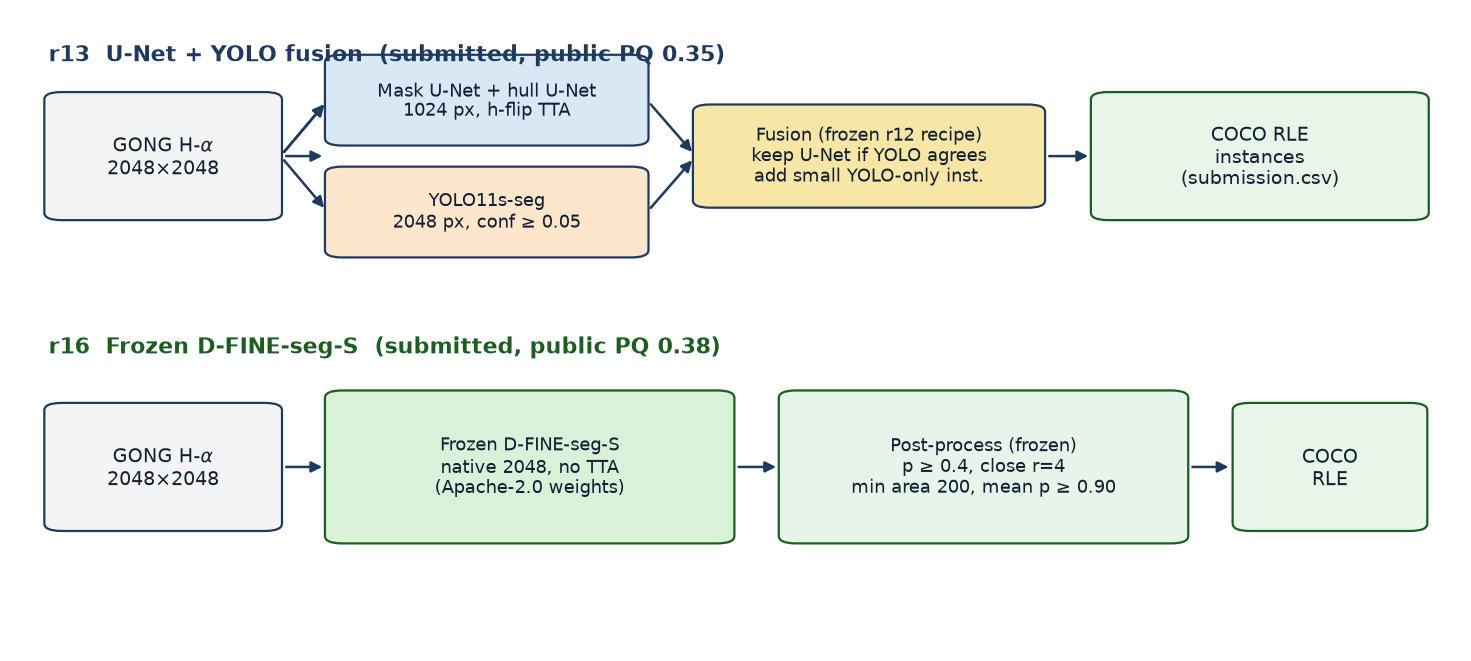
\includegraphics[width=\textwidth]{fig0_pipeline.png}
  \Description{Flow diagram of the r13 U-Net plus YOLO fusion pipeline and the r16 frozen D-FINE-seg-S pipeline, both ending in COCO RLE instances.}
  \caption{End-to-end pipelines for the two submitted entries. Top: r13 U-Net + YOLO fusion. Bottom: r16 frozen D-FINE-seg-S. Both write one COCO RLE per instance in the organizers' \texttt{submission.csv} schema.}
  \label{fig:pipeline}
\end{figure*}

\section{Evaluation}
\label{sec:eval}

\paragraph{Protocol.}
The official metric is Panoptic Quality [3]. We score holdouts with a verbatim port of the organizers' self-evaluation function \texttt{get\_pq\_score}:\footnote{\url{https://www.kaggle.com/code/azimahmadzadeh/self-evaluation-notebook}} a ground-truth and predicted filament match when IoU $> 0.5$, and
\[
\mathrm{PQ}=\frac{\sum_{\mathrm{TP}}\mathrm{IoU}}{|\mathrm{TP}|+\tfrac12|\mathrm{FP}|+\tfrac12|\mathrm{FN}|},
\]
pooled over annotator-images (each annotator's view of a file is a separate row). We compared the port against the published notebook; the matching rule and formula are the same. A \texttt{metrics.py} file shipped with D-FINE-seg uses pycocotools IoU and $\mathrm{FP}=n_{\mathrm{pred}}-\mathrm{TP}$, which agrees when matches at IoU $>0.5$ are unique, as the organizers assume. The numbers below do \emph{not} use that file.

Uncertainty is reported in two related ways, both from saved per-id $(\mathrm{TP},\mathrm{FP},\mathrm{FN},\sum\mathrm{IoU})$ rows and 10{,}000 resamples of annotator-image ids (seed 0), with no new inference. (i)~For the official metric we recompute \emph{pooled} PQ (and paired gain) on each resample and give a percentile 95\% confidence interval (CI). (ii)~Our pre-registered margin gate bootstraps the \emph{mean of per-image PQ differences}, with $\alpha=0.05/k$ after $k$ uses of the holdout.

\paragraph{Main results.}
Table~\ref{tab:main} and Figure~\ref{fig:ci} collect the holdout scores. On the fresh 201-id holdout, fusion reached PQ 0.4092 versus 0.3846 for the U-Net alone, a gain of $+0.0246$ against a pre-set bar of $+0.015$. Segmentation quality was essentially unchanged (SQ $0.667$ vs.\ $0.669$); the gain is in recognition quality (RQ $0.613$ vs.\ $0.575$), i.e.\ 80 additional matched filaments with only seven more false positives. The pooled-PQ bootstrap 95\% CI for the gain is $[0.0153,0.0342]$. The pre-registered margin gate ($k=1$) gave a 95\% lower bound of $+0.020$ on the mean per-image difference, and passed. Public PQ was 0.35 (submission 58336268), up from 0.33--0.34 for our earlier U-Net-only entries.

On the leak-free 46-id slice, frozen D-FINE-seg-S scored 0.4321 versus 0.4038 for the r13 recipe (gain $+0.0282$; TP 205 vs.\ 201, FP 123 vs.\ 157, FN 108 vs.\ 112). Gate 1 (the $+0.015$ bar) passed. Gate 2 blocked: with inherited $k=4$, the 98.75\% lower bound on the mean per-image difference was $-0.0118$ (mean $+0.0325$). The corresponding pooled-PQ 95\% CI for the gain is $[-0.0009,0.0576]$ and includes zero---the 46-id slice is too small to confirm the point-estimate gain. The file was nevertheless submitted under an explicit override (submission 58424634) and scored 0.38 on the public board, $+0.03$ over r13, short of a written public-gain line of 0.39. After scoring, the team stood at rank 506 of about 1{,}566.

\begin{table*}[t]
  \caption{Holdout PQ (official pooled \texttt{get\_pq\_score}) with image-resampled 95\% CIs. The two blocks are different row sets and are not comparable as a single ladder. Public scores are Kaggle's two-decimal board values.}
  \label{tab:main}
  \centering
  \small
  \begin{tabular}{@{}l l r c c c c@{}}
    \toprule
    Method & Holdout & PQ & 95\% CI & SQ / RQ & TP / FP / FN & Public \\
    \midrule
    U-Net only (r5 recipe) & fresh13, 201 ids & 0.3846 & $[0.364,0.405]$ & 0.669 / 0.575 & 789 / 587 / 581 & 0.33--0.34 \\
    U-Net+YOLO fusion (r13) & fresh13, 201 ids & 0.4092 & $[0.390,0.427]$ & 0.667 / 0.613 & 869 / 594 / 501 & 0.35 \\
    \midrule
    r13 recipe replayed & 46-id slice & 0.4038 & $[0.360,0.444]$ & 0.674 / 0.599 & 201 / 157 / 112 & --- \\
    Frozen D-FINE-seg-S (r16) & 46-id slice & 0.4321 & $[0.384,0.477]$ & 0.675 / 0.640 & 205 / 123 / 108 & 0.38 \\
    \bottomrule
  \end{tabular}
\end{table*}

\begin{figure}[t]
  \centering
  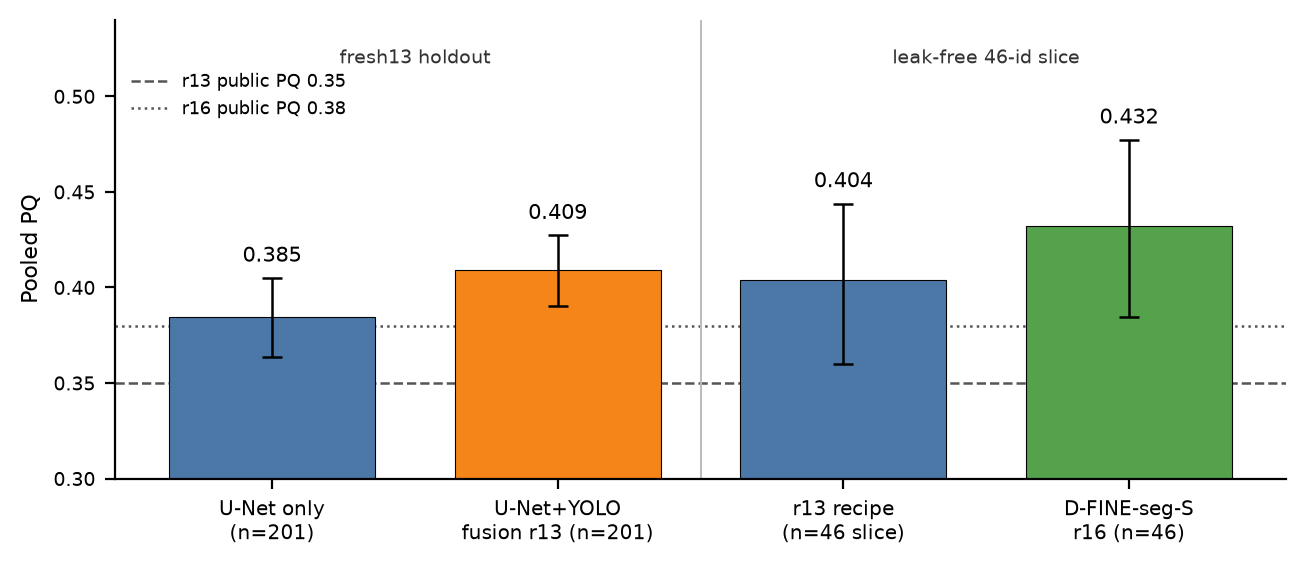
\includegraphics[width=\columnwidth]{fig3_pq_ci.png}
  \Description{Bar chart of pooled holdout panoptic quality for four methods with 95 percent bootstrap confidence intervals and reference lines at the public scores 0.35 and 0.38.}
  \caption{Pooled holdout PQ with 95\% bootstrap CIs from 10{,}000 resamples of annotator-image ids. Dashed and dotted lines mark our public scores (no public CI is available).}
  \label{fig:ci}
\end{figure}

\paragraph{Where the r13 gain comes from.}
Table~\ref{tab:diag} and Figure~\ref{fig:hist} summarize best-match IoU and Dice for every ground-truth filament on the 201-id holdout. Mean matched-pair IoU stays about 0.67. Fusion finds more filaments: 74 fewer ground-truth filaments have no overlapping prediction (175 vs.\ 249), and one-to-many fragmentation falls from 70 to 49, at a cost of six more many-to-one merges. Figure~\ref{fig:overlay} shows a holdout image with the median r13 per-image PQ (0.43): most misses are small, faint filaments. On the 120 files with more than one annotator, annotator-versus-annotator PQ is only 0.329 (SQ 0.63), so our SQ is already near that agreement ceiling; remaining controllable loss is mostly counting error.

\begin{table}[t]
  \caption{Best-match IoU/Dice diagnostics on the 201-id fresh holdout (1{,}370 ground-truth filaments).}
  \label{tab:diag}
  \centering
  \small
  \begin{tabular}{@{}l cc@{}}
    \toprule
     & U-Net only & Fusion (r13) \\
    \midrule
    Predicted instances & 1{,}376 & 1{,}463 \\
    Best-match IoU mean (median) & 0.471 (0.562) & 0.508 (0.590) \\
    Best-match Dice mean (median) & 0.584 (0.719) & 0.628 (0.742) \\
    Matched-pair IoU / Dice mean & 0.669 / 0.799 & 0.667 / 0.797 \\
    GT with no overlap & 249 & 175 \\
    One-to-many (GT; IoU$>0$) & 70 & 49 \\
    Many-to-one (pred; IoU$>0$) & 43 & 49 \\
    \bottomrule
  \end{tabular}
\end{table}

\begin{figure*}[t]
  \centering
  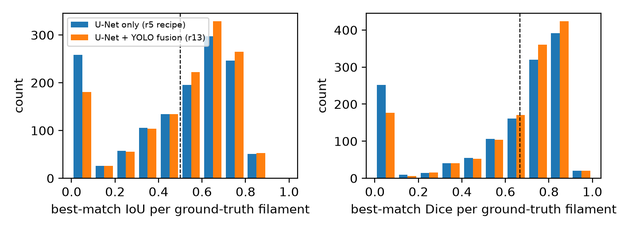
\includegraphics[width=0.92\textwidth]{fig1_iou_dice_hist.png}
  \Description{Side-by-side histograms of best-match IoU and Dice per ground-truth filament, comparing U-Net only with the r13 fusion.}
  \caption{Best-match IoU (left) and Dice (right) per ground-truth filament on the fresh 201-id holdout. The dashed line is the matching threshold (IoU 0.5, equivalent to Dice $2/3$).}
  \label{fig:hist}
\end{figure*}

\begin{figure*}[t]
  \centering
  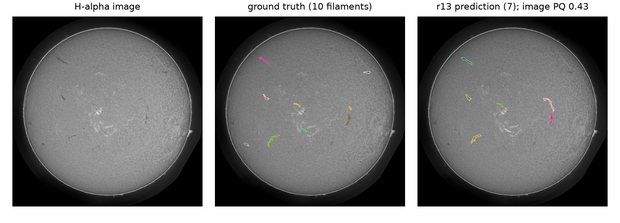
\includegraphics[width=0.92\textwidth]{fig2_overlay_median.png}
  \Description{Three-panel figure of a holdout H-alpha image, its ground-truth filaments, and the r13 predictions on an image with median per-image PQ of 0.43.}
  \caption{A holdout image with the median r13 per-image PQ (0.43): 6 matches, 1 false positive, 4 misses. Most misses are small, faint filaments.}
  \label{fig:overlay}
\end{figure*}

\paragraph{What did not help.}
Each row in Table~\ref{tab:neg} had a fixed pass bar, failed it, and was not submitted. In particular, replacing YOLO11s with YOLO11m inside the r13 recipe slightly hurt, and a crop U-Net refiner on r13 instances gained only $+0.0048$ (bar $+0.015$); its margin gate at $k=3$ also blocked (lower bound $-0.0022$).

\begin{table}[t]
  \caption{Pre-registered rounds that did not pass their bar and were not submitted. Holdout PQ is the official pooled score.}
  \label{tab:neg}
  \centering
  \small
  \begin{tabular}{@{}l p{0.36\columnwidth} p{0.28\columnwidth}@{}}
    \toprule
    Round & Change & Holdout result \\
    \midrule
    v5/v7 & Mask R-CNN [8] and U-Net hybrids & 0.358--0.377 vs.\ 0.400 \\
    r7 & Centreline + seeded watershed & 0.4005 vs.\ 0.4053 \\
    r8 & 1024-px tiles at native 2048 & 0.4086 vs.\ 0.4095 \\
    r10 & YOLO11s-seg alone & 0.4002 vs.\ 0.4095 \\
    r11/r12 & Fusion on a reused holdout & point bar ok; reuse gate blocked \\
    r14 & YOLO11m in the r13 recipe & 0.4061 vs.\ 0.4092 \\
    r15 & Crop U-Net refiner & 0.4140 vs.\ 0.4092 \\
    \bottomrule
  \end{tabular}
\end{table}

\paragraph{Strengths, weaknesses, and improvements.}
Fusion is a cheap, interpretable way to cut missed filaments without hurting match quality, and it was confirmed on a fresh holdout with a CI that excludes zero. The frozen D-FINE-seg-S recipe is simpler, reduced false positives on the 46-id slice, and is our best public score (0.38). Weaknesses: the holdout-to-public gap (0.41 vs.\ 0.35 for r13; a wide CI for r16) shows that even a file-grouped holdout is optimistic; the only leak-free slice for the published D-FINE weights is too small for the uncertainty gate to pass; and 175 ground-truth filaments still have no overlapping r13 prediction, almost all of them small and faint. Honest next steps are to retrain D-FINE-seg-S on the r13 split (excluding all of \texttt{fresh13}) and score the full 201 ids, to build a larger holdout earlier in a competition, and to try a $k$-fold ensemble rather than a higher-capacity YOLO or a crop refiner, both of which already failed their bars.

\section*{Conclusion}
We submitted a U-Net + YOLO fusion (public PQ 0.35) and a frozen D-FINE-seg-S model (public PQ 0.38). The fusion gain is a confirmed recall improvement on a fresh 201-id holdout. The D-FINE point-estimate gain on 46 leak-free ids did not pass a reuse-adjusted uncertainty gate, but the submitted file is our best public score. Remaining errors are mostly small, faint filaments, and the holdout remains optimistic relative to the public board.

\section{Acknowledgment}
The organization of the Filament Segmentation Challenge 2026 is
partially supported by the U.S. National Science Foundation (NSF)
under Grant No. 2209912 and 2433781, directorate for Computer and
Information Science and Engineering (CSE), and Office of Advanced
Cyberinfrastructure (OAC), and Grant No. 2511630, AST Division
Of Astronomical Sciences and MPS Directorate for Mathematical
and Physical Sciences.

The Filament Segmentation Challenge 2026 is sponsored by the
U.S. National Science Foundation (NSF) National Solar Observatory
(NSO).

This work utilizes GONG data obtained by the NSO Integrated
Synoptic Program, managed by the National Solar Observatory,
which is operated by the Association of Universities for Research
in Astronomy (AURA), Inc.\ under a cooperative agreement with
the National Science Foundation and with contribution from the
National Oceanic and Atmospheric Administration. The GONG
network of instruments is hosted by the Big Bear Solar Observatory,
High Altitude Observatory, Learmonth Solar Observatory, Udaipur
Solar Observatory, Instituto de Astrof\'isica de Canarias, and Cerro
Tololo Interamerican Observatory.

\begin{thebibliography}{10}

\bibitem{ahmadzadeh2024}
Azim Ahmadzadeh, Rohan Adhyapak, Kartik Chaurasiya, Laxmi Alekhya Nagubandi, V. Aparna, Petrus C. Martens, Alexei Pevtsov, Luca Bertello, Alexander Pevtsov, Naomi Douglas, Samuel McDonald, Apaar Bawa, Eugene Kang, Riley Wu, Dustin J. Kempton, Aya Abdelkarem, Patrick M. Copeland, and Sri Harsha Seelamneni. 2024. A dataset of manually annotated filaments from H-alpha observations. In \emph{Nature Scientific Data} (\emph{Nature Scientific Data}, Vol.~11). Springer, Article 1031, 1031 pages. doi:10.1038/s41597-024-03876-y

\bibitem{filament2026}
Azim Ahmadzadeh, Dustin J. Kempton, Qin Li, and Alexei A. Pevtsov. 2026. Solar Filament Segmentation Challenge 2026. \url{https://kaggle.com/competitions/filament-segmentation-2026}. Kaggle.

\bibitem{kirillov2019pq}
Alexander Kirillov, Kaiming He, Ross Girshick, Carsten Rother, and Piotr Doll\'ar. 2019. Panoptic Segmentation. In \emph{IEEE/CVF Conference on Computer Vision and Pattern Recognition (CVPR)}. 9404--9413.

\bibitem{ronneberger2015unet}
Olaf Ronneberger, Philipp Fischer, and Thomas Brox. 2015. U-Net: Convolutional Networks for Biomedical Image Segmentation. In \emph{Medical Image Computing and Computer-Assisted Intervention (MICCAI)}. Springer, 234--241.

\bibitem{jocher2024yolo}
Glenn Jocher and Jing Qiu. 2024. Ultralytics YOLO11. \url{https://github.com/ultralytics/ultralytics}.

\bibitem{peng2025dfine}
Yansong Peng, Hebei Li, Peixi Wu, Yueyi Zhang, Xiaoyan Sun, and Feng Wu. 2025. D-FINE: Redefine Regression Task of DETRs as Fine-grained Distribution Refinement. In \emph{The Thirteenth International Conference on Learning Representations}.

\bibitem{argoha2026dfine}
ArgoHA. 2026. solar-filament-dfine-seg. \url{https://github.com/ArgoHA/solar-filament-dfine-seg}. Apache-2.0.

\bibitem{he2017maskrcnn}
Kaiming He, Georgia Gkioxari, Piotr Doll\'ar, and Ross Girshick. 2017. Mask R-CNN. In \emph{IEEE International Conference on Computer Vision (ICCV)}. 2961--2969.

\end{thebibliography}
\end{document}
